\documentclass[tikz,border=3pt]{standalone}
\usepackage[utf8]{inputenc}
\usepackage[T1]{fontenc}
\usepackage{lmodern}
\renewcommand{\familydefault}{\sfdefault}
\usepackage{sansmath}\sansmath
\usepackage{chemfig}
\usepackage{pgfplots}\pgfplotsset{compat=1.18,/pgf/number format/use comma,/pgf/number format/1000 sep={.}}
\usetikzlibrary{arrows.meta,calc,positioning,decorations.pathmorphing,patterns}
% paleta del sitio
\definecolor{nar}{HTML}{E8680C}\definecolor{narc}{HTML}{FFB35C}\definecolor{hielo}{HTML}{FFF3E8}
\definecolor{tinta}{HTML}{1D1D1F}\definecolor{gris}{HTML}{6E6E73}\definecolor{lila}{HTML}{7C5CF0}
\definecolor{azul}{HTML}{2F6FD6}\definecolor{menta}{HTML}{17A673}\definecolor{coral}{HTML}{E8342A}
\tikzset{cel/.style={draw=gris,fill=hielo,line width=0.9pt},nuc/.style={draw=gris!70,line width=0.6pt},
fib/.style={gris!55,line width=0.35pt},eti/.style={font=\footnotesize,text=tinta,align=center},
num/.style={circle,draw=nar,fill=white,text=nar,font=\small\bfseries,inner sep=1.2pt,minimum size=13pt},
fl/.style={-{Stealth[length=2.6mm]},gris,line width=0.9pt}}
\begin{document}
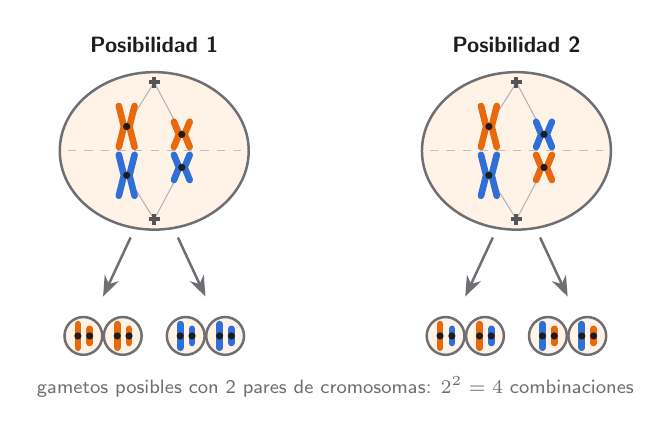
\begin{tikzpicture}[font=\small]
\draw[cel] (0,0) ellipse (1.2 and 1);
\draw[gris!45,dashed] (-1.1,0)--(1.1,0);
\draw[fib] (0,0.87)--(-0.35,0.31);
\draw[fib] (0,0.87)--(0.35,0.21);
\draw[fib] (0,-0.87)--(-0.35,-0.31);
\draw[fib] (0,-0.87)--(0.35,-0.21);
\begin{scope}[shift={(-0.35,0.31)},rotate=0]\draw[nar,line width=2.4pt,line cap=round,line join=round] (-0.1,0.26)--(-0.035,0)--(-0.1,-0.26);\end{scope}
\begin{scope}[shift={(-0.35,0.31)},rotate=0]\draw[nar,line width=2.4pt,line cap=round,line join=round] (0.1,0.26)--(0.035,0)--(0.1,-0.26);\end{scope}
\fill[tinta] (-0.35,0.31) circle (1.3pt);
\begin{scope}[shift={(0.35,0.21)},rotate=0]\draw[nar,line width=2.4pt,line cap=round,line join=round] (-0.1,0.16)--(-0.035,0)--(-0.1,-0.16);\end{scope}
\begin{scope}[shift={(0.35,0.21)},rotate=0]\draw[nar,line width=2.4pt,line cap=round,line join=round] (0.1,0.16)--(0.035,0)--(0.1,-0.16);\end{scope}
\fill[tinta] (0.35,0.21) circle (1.3pt);
\begin{scope}[shift={(-0.35,-0.31)},rotate=0]\draw[azul,line width=2.4pt,line cap=round,line join=round] (-0.1,0.26)--(-0.035,0)--(-0.1,-0.26);\end{scope}
\begin{scope}[shift={(-0.35,-0.31)},rotate=0]\draw[azul,line width=2.4pt,line cap=round,line join=round] (0.1,0.26)--(0.035,0)--(0.1,-0.26);\end{scope}
\fill[tinta] (-0.35,-0.31) circle (1.3pt);
\begin{scope}[shift={(0.35,-0.21)},rotate=0]\draw[azul,line width=2.4pt,line cap=round,line join=round] (-0.1,0.16)--(-0.035,0)--(-0.1,-0.16);\end{scope}
\begin{scope}[shift={(0.35,-0.21)},rotate=0]\draw[azul,line width=2.4pt,line cap=round,line join=round] (0.1,0.16)--(0.035,0)--(0.1,-0.16);\end{scope}
\fill[tinta] (0.35,-0.21) circle (1.3pt);
\fill[tinta!75] (-0.07,0.845) rectangle (0.07,0.895);\fill[tinta!75] (-0.025,0.8) rectangle (0.025,0.94);
\fill[tinta!75] (-0.07,-0.895) rectangle (0.07,-0.845);\fill[tinta!75] (-0.025,-0.94) rectangle (0.025,-0.8);
\node[eti] at (0,1.35) {\textbf{Posibilidad 1}};
\draw[fl] (-0.3,-1.1)--(-0.65,-1.85);
\draw[cel] (-0.9,-2.35) circle (0.24);
\begin{scope}[shift={(-0.97,-2.35)},rotate=0]\draw[nar,line width=2.4pt,line cap=round,line join=round] (0,0.15)--(0,0)--(0,-0.15);\end{scope}
\fill[tinta] (-0.97,-2.35) circle (1.3pt);
\begin{scope}[shift={(-0.82,-2.35)},rotate=0]\draw[nar,line width=2.4pt,line cap=round,line join=round] (0,0.09)--(0,0)--(0,-0.09);\end{scope}
\fill[tinta] (-0.82,-2.35) circle (1.3pt);
\draw[cel] (-0.4,-2.35) circle (0.24);
\begin{scope}[shift={(-0.47,-2.35)},rotate=0]\draw[nar,line width=2.4pt,line cap=round,line join=round] (0,0.15)--(0,0)--(0,-0.15);\end{scope}
\fill[tinta] (-0.47,-2.35) circle (1.3pt);
\begin{scope}[shift={(-0.32,-2.35)},rotate=0]\draw[nar,line width=2.4pt,line cap=round,line join=round] (0,0.09)--(0,0)--(0,-0.09);\end{scope}
\fill[tinta] (-0.32,-2.35) circle (1.3pt);
\draw[fl] (0.3,-1.1)--(0.65,-1.85);
\draw[cel] (0.4,-2.35) circle (0.24);
\begin{scope}[shift={(0.33,-2.35)},rotate=0]\draw[azul,line width=2.4pt,line cap=round,line join=round] (0,0.15)--(0,0)--(0,-0.15);\end{scope}
\fill[tinta] (0.33,-2.35) circle (1.3pt);
\begin{scope}[shift={(0.48,-2.35)},rotate=0]\draw[azul,line width=2.4pt,line cap=round,line join=round] (0,0.09)--(0,0)--(0,-0.09);\end{scope}
\fill[tinta] (0.48,-2.35) circle (1.3pt);
\draw[cel] (0.9,-2.35) circle (0.24);
\begin{scope}[shift={(0.83,-2.35)},rotate=0]\draw[azul,line width=2.4pt,line cap=round,line join=round] (0,0.15)--(0,0)--(0,-0.15);\end{scope}
\fill[tinta] (0.83,-2.35) circle (1.3pt);
\begin{scope}[shift={(0.98,-2.35)},rotate=0]\draw[azul,line width=2.4pt,line cap=round,line join=round] (0,0.09)--(0,0)--(0,-0.09);\end{scope}
\fill[tinta] (0.98,-2.35) circle (1.3pt);
\draw[cel] (4.6,0) ellipse (1.2 and 1);
\draw[gris!45,dashed] (3.5,0)--(5.7,0);
\draw[fib] (4.6,0.87)--(4.25,0.31);
\draw[fib] (4.6,0.87)--(4.95,0.21);
\draw[fib] (4.6,-0.87)--(4.25,-0.31);
\draw[fib] (4.6,-0.87)--(4.95,-0.21);
\begin{scope}[shift={(4.25,0.31)},rotate=0]\draw[nar,line width=2.4pt,line cap=round,line join=round] (-0.1,0.26)--(-0.035,0)--(-0.1,-0.26);\end{scope}
\begin{scope}[shift={(4.25,0.31)},rotate=0]\draw[nar,line width=2.4pt,line cap=round,line join=round] (0.1,0.26)--(0.035,0)--(0.1,-0.26);\end{scope}
\fill[tinta] (4.25,0.31) circle (1.3pt);
\begin{scope}[shift={(4.95,0.21)},rotate=0]\draw[azul,line width=2.4pt,line cap=round,line join=round] (-0.1,0.16)--(-0.035,0)--(-0.1,-0.16);\end{scope}
\begin{scope}[shift={(4.95,0.21)},rotate=0]\draw[azul,line width=2.4pt,line cap=round,line join=round] (0.1,0.16)--(0.035,0)--(0.1,-0.16);\end{scope}
\fill[tinta] (4.95,0.21) circle (1.3pt);
\begin{scope}[shift={(4.25,-0.31)},rotate=0]\draw[azul,line width=2.4pt,line cap=round,line join=round] (-0.1,0.26)--(-0.035,0)--(-0.1,-0.26);\end{scope}
\begin{scope}[shift={(4.25,-0.31)},rotate=0]\draw[azul,line width=2.4pt,line cap=round,line join=round] (0.1,0.26)--(0.035,0)--(0.1,-0.26);\end{scope}
\fill[tinta] (4.25,-0.31) circle (1.3pt);
\begin{scope}[shift={(4.95,-0.21)},rotate=0]\draw[nar,line width=2.4pt,line cap=round,line join=round] (-0.1,0.16)--(-0.035,0)--(-0.1,-0.16);\end{scope}
\begin{scope}[shift={(4.95,-0.21)},rotate=0]\draw[nar,line width=2.4pt,line cap=round,line join=round] (0.1,0.16)--(0.035,0)--(0.1,-0.16);\end{scope}
\fill[tinta] (4.95,-0.21) circle (1.3pt);
\fill[tinta!75] (4.53,0.845) rectangle (4.67,0.895);\fill[tinta!75] (4.575,0.8) rectangle (4.625,0.94);
\fill[tinta!75] (4.53,-0.895) rectangle (4.67,-0.845);\fill[tinta!75] (4.575,-0.94) rectangle (4.625,-0.8);
\node[eti] at (4.6,1.35) {\textbf{Posibilidad 2}};
\draw[fl] (4.3,-1.1)--(3.95,-1.85);
\draw[cel] (3.7,-2.35) circle (0.24);
\begin{scope}[shift={(3.63,-2.35)},rotate=0]\draw[nar,line width=2.4pt,line cap=round,line join=round] (0,0.15)--(0,0)--(0,-0.15);\end{scope}
\fill[tinta] (3.63,-2.35) circle (1.3pt);
\begin{scope}[shift={(3.78,-2.35)},rotate=0]\draw[azul,line width=2.4pt,line cap=round,line join=round] (0,0.09)--(0,0)--(0,-0.09);\end{scope}
\fill[tinta] (3.78,-2.35) circle (1.3pt);
\draw[cel] (4.2,-2.35) circle (0.24);
\begin{scope}[shift={(4.13,-2.35)},rotate=0]\draw[nar,line width=2.4pt,line cap=round,line join=round] (0,0.15)--(0,0)--(0,-0.15);\end{scope}
\fill[tinta] (4.13,-2.35) circle (1.3pt);
\begin{scope}[shift={(4.28,-2.35)},rotate=0]\draw[azul,line width=2.4pt,line cap=round,line join=round] (0,0.09)--(0,0)--(0,-0.09);\end{scope}
\fill[tinta] (4.28,-2.35) circle (1.3pt);
\draw[fl] (4.9,-1.1)--(5.25,-1.85);
\draw[cel] (5,-2.35) circle (0.24);
\begin{scope}[shift={(4.93,-2.35)},rotate=0]\draw[azul,line width=2.4pt,line cap=round,line join=round] (0,0.15)--(0,0)--(0,-0.15);\end{scope}
\fill[tinta] (4.93,-2.35) circle (1.3pt);
\begin{scope}[shift={(5.08,-2.35)},rotate=0]\draw[nar,line width=2.4pt,line cap=round,line join=round] (0,0.09)--(0,0)--(0,-0.09);\end{scope}
\fill[tinta] (5.08,-2.35) circle (1.3pt);
\draw[cel] (5.5,-2.35) circle (0.24);
\begin{scope}[shift={(5.43,-2.35)},rotate=0]\draw[azul,line width=2.4pt,line cap=round,line join=round] (0,0.15)--(0,0)--(0,-0.15);\end{scope}
\fill[tinta] (5.43,-2.35) circle (1.3pt);
\begin{scope}[shift={(5.58,-2.35)},rotate=0]\draw[nar,line width=2.4pt,line cap=round,line join=round] (0,0.09)--(0,0)--(0,-0.09);\end{scope}
\fill[tinta] (5.58,-2.35) circle (1.3pt);
\node[eti,font=\scriptsize,text=gris] at (2.3,-3) {gametos posibles con 2 pares de cromosomas: $2^2 = 4$ combinaciones};
\end{tikzpicture}
\end{document}
